\documentclass[tikz,border=12pt]{standalone}
\usepackage{lmodern}
\usepackage[T1]{fontenc}
\usetikzlibrary{calc}

% Edit these expressions to change the labels on each side.
\newcommand{\BottomLabel}{$dx=\sqrt{\mathrm{d}x_i \mathrm{d}x^{i}} = v \tau$}
\newcommand{\VerticalLabel}{$\mathrm{d}y= \tau \frac{v^{2}}{\sqrt{c^{2} - v^{2}}}$}
\newcommand{\HypotenuseLabel}{$\mathrm{d}x^{\left( U \right)}= \sqrt{\mathrm{d}x_i \mathrm{d}x^{i}} \tau \gamma$}

\begin{document}
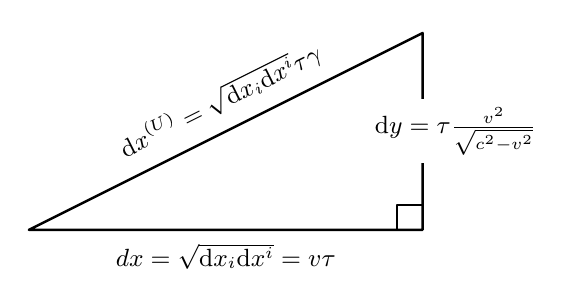
\begin{tikzpicture}[
  line cap=round,
  line join=round,
  font=\sffamily,
  triangle edge/.style={draw=black,line width=0.9pt},
  side label/.style={font=\small,text=black,fill=white,inner sep=3pt}
]
  % Right triangle, with the perpendicular legs along the page axes.
  \coordinate (A) at (0,0);
  \coordinate (B) at (5,0);
  \coordinate (C) at (5,2.5);

  \draw[triangle edge] (A) -- (B) -- (C) -- cycle;

  % Conventional right-angle marker at the corner between the legs.
  \draw[line width=0.7pt] (4.68,0) -- (4.68,0.32) -- (5,0.32);

  % Labels follow the orientation of their respective sides.
  \node[side label] at (2.5,-0.34) {\BottomLabel};
  \node[side label] at (5.42,1.25) {\VerticalLabel};
  \node[side label,rotate=26.565] at (2.43,1.64) {\HypotenuseLabel};
\end{tikzpicture}
\end{document}
